\chapter{Combinatorics}

Combinatorics is, loosely, the mathematics of counting and 
permutations. These notes are based on lectures given by Shiyun 
Wang at the University of Minnesota during the Fall 2023 semester.

%%%%%%%%%%%%%%%%%%%%%%%%%%%%%%%%%%%%%%%%%%%%%%%%%%%%%%%%%%%%%%%%%%

\newpage

\section{The Pigeonhole Principle}\index{pigeonhole principle}

Main idea: If we put 4 pigeons into 3 pigeonholes, at least one 
pigeon will have to share.

\begin{marginfigure}[.2in]
	\includegraphics[scale=.1]{TooManyPigeons.jpg}
	\caption{Too many pigeons.}
\end{marginfigure}

\begin{definition}[Pigeonhole Principle]
	Let $n$, $k$ be positive integers with $n > k$. Suppose that we 
	place $n$ identical balls into $k$ identical boxes. Then there 
	will be at least one box in which we place at least two balls.
	
	More generally, if we have $n$ identical balls and $m$ boxes 
	with $n > rm$, then there will be at least one box with $r + 1$ 
	balls.
\end{definition}

\begin{marginfigure}[.4in]
	\centering
	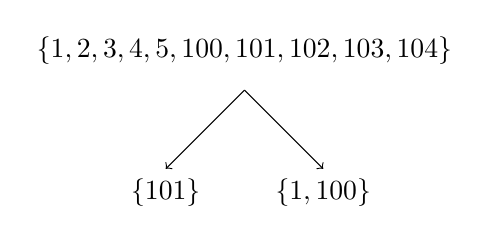
\begin{tikzpicture}
		\node (0,0) {$\{ 1, 2, 3, 4, 5, 100, 101, 102, 103, 104 
			\}$};
		\draw[->] (0,-.5) -- (-1,-1.5);
		\draw[->] (0,-.5) -- (1,-1.5);
		\node[below] at (-1,-1.5) {$\{ 101 \}$};
		\node[below] at (1,-1.5) {$\{ 1, 100 \}$};
	\end{tikzpicture}
	\caption{An example of a 10-digit set split into two disjoint 
		subsets with the same sum.}\label{pigeon}
\end{marginfigure}

\begin{example}
	Given ten distinct positive integers less than 107, there exist 
	two disjoint subsets with the same sum. As an illustration, 
	consider Figure \ref{pigeon}.
	
	\begin{proof}
		The largest sum possible would be $\sum_{i=97}^{106} i = 
		1015$. We consider the possible sums of our subsets to be 
		the boxes referred to by the Pigeonhole Principle, and so 
		we have 1016 boxes (the subset being the empty set 
		corresponds to the box with sum of 0). But for a set 
		containing 10 numbers, we have $2^{10} = 1024$ subsets. By 
		the pigeonhole principle, at least two of these subsets 
		have the same sum since $1024 > 1016$. If they are not 
		disjoint, remove their intersection and they will still 
		have the same sum.
	\end{proof}
\end{example}

\begin{marginfigure}[1in]
	\centering
	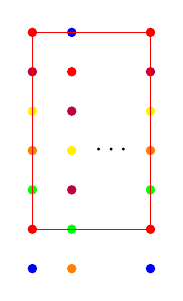
\begin{tikzpicture}
		\filldraw[blue] (0,0) circle (1.5pt);
		\filldraw[red] (0,.5) circle (1.5pt);
		\filldraw[green] (0,1) circle (1.5pt);
		\filldraw[orange] (0,1.5) circle (1.5pt);
		\filldraw[yellow] (0,2) circle (1.5pt);
		\filldraw[purple] (0,2.5) circle (1.5pt);
		\filldraw[red] (0,3) circle (1.5pt);
		
		\filldraw[orange] (.5,0) circle (1.5pt);
		\filldraw[green] (.5,.5) circle (1.5pt);
		\filldraw[purple] (.5,1) circle (1.5pt);
		\filldraw[yellow] (.5,1.5) circle (1.5pt);
		\filldraw[purple] (.5,2) circle (1.5pt);
		\filldraw[red] (.5,2.5) circle (1.5pt);
		\filldraw[blue] (.5,3) circle (1.5pt);
		
		\node at (1,1.5) {$\cdots$};
		
		\filldraw[blue] (1.5,0) circle (1.5pt);
		\filldraw[red] (1.5,.5) circle (1.5pt);
		\filldraw[green] (1.5,1) circle (1.5pt);
		\filldraw[orange] (1.5,1.5) circle (1.5pt);
		\filldraw[yellow] (1.5,2) circle (1.5pt);
		\filldraw[purple] (1.5,2.5) circle (1.5pt);
		\filldraw[red] (1.5,3) circle (1.5pt);
		
		\draw[red] (0,.5) -- (1.5,.5) -- (1.5,3) -- (0,3) -- (0,.5);
	\end{tikzpicture}
	\caption{Eventually the coloring of neighboring sets of seven 
	vertical vertices will have to repeat, yielding a rectangle 
	with monochromatic vertices.}\label{mono rect}
\end{marginfigure}

\begin{example}
	Consider $\reals^2$ restricted to integer coordinates. Show 
	there is no way to assign one of six colors to each vertex such 
	that there does not exist a rectangle whose vertices are 
	monochromatic.
	
	\begin{proof}
		I present a simplified version of the proof from class. 
		Consider a vertical column of seven vertices. Since there 
		are only 6 colors, any coloring of these seven vertices 
		will result in a repeated color. This repeated color is red 
		in the first vertical column of Figure \ref{mono rect}. 
		There are a finite number, let's say $k$, of ways to color 
		seven vertical vertices without repeating the coloring in 
		our first column. So if we pick $k+1$ neighboring columns 
		of seven vertices, then by the pigeonhole principle at 
		least two columns must share the same coloring. This will 
		yield a rectangle with monochromatic vertices, drawn in red 
		in Figure \ref{mono rect}.
	\end{proof}
\end{example}

































